\textcolor{ubuntu_orange}{Panel menu} łączy w sobie kilka funkcji i to, co od razu rzuca się w oczy, to umieszczony po prawej stronie \textcolor{ubuntu_orange}{obszar powiadamiania}, zwany inaczej obszarem wskaźników.

\begin{center}
	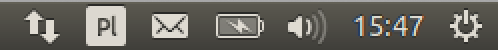
\includegraphics[width=\linewidth]{images/unity_menu_bar.png}
\end{center}

Część wskaźników widoczna jest zaraz po zainstalowaniu systemu, inne można włączyć dodatkowo. Niektóre aplikacje po zainstalowaniu dodają lub umożliwiają dodanie własnych wskaźników do obszaru powiadamiania. Najczęściej stosowane i domyślnie dostępne w Unity wskaźniki, to:
\begin{description}
\item[
\includegraphics{images/unity_wskaznik_siec.png}]\textcolor{ubuntu_orange}{Wskaźnik połączeń sieciowych} --- informuje o stanie połączenia z siecią. Kliknięcie wywołuje opcje modyfikacji połączenia z internetem.
\item[
\includegraphics{images/unity_wskaznik_klawiatura.png}]\textcolor{ubuntu_orange}{Wskaźnik klawiatury} --- informuje o aktualnie używanym układzie klawiatury. Klikając go możesz zmienić układ klawiatury.
\item[
\includegraphics{images/unity_wskaznik_wiadomosci.png}]\textcolor{ubuntu_orange}{Wskaźnik wiadomości} --- informuje o przychodzących wiadomościach. Ten wskaźnik integruje się z komunikatorami internetowymi i zmienia kolor, gdy otrzymasz nową wiadomość. Pozwala także sterować komunikatorem, np. zmienić status lub wywołać okno główne.
\item[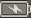
\includegraphics{images/unity_wskaznik_zasilanie.png}]\textcolor{ubuntu_orange}{Wskaźnik zasilania i poziomu akumulatora} --- informuje o stanie stanie naładowania akumulatora oraz o dostępnym zasilaniu (akumulator/sieć). Ten wskaźnik nie jest wyświetlany, jesli komputer nie ma baterii. Kliknięcie wskaźnika otwiera menu zasilania.
\item[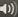
\includegraphics{images/unity_wskaznik_dzwiek.png}]\textcolor{ubuntu_orange}{Wskaźnik ustawień dźwięku} --- informuje o głośności wyjścia audio. Jeżeli kursor myszy znajduje się nad tym wskaźnikiem, to poruszając kółkiem myszy możesz zmieniać głośność. Kliknięcie wskaźnika otwiera menu ustawień dźwięku oraz menu sterownia odtwarzaczem muzyki (pozwala np. go uruchomić lub zatrzymać, zmienić utwór, wyświetlić okładkę i informacje o aktualnie odtwarzanym pliku,a także włączyć listę odtwarzania).
\item[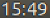
\includegraphics{images/unity_wskaznik_zegar.png}]\textcolor{ubuntu_orange}{Zegar} --- wyświetla aktualną datę i czas. Kliknięcie otwiera kalendarz.
\item[
\includegraphics{images/unity_wskaznik_system.png}]\textcolor{ubuntu_orange}{Wskaźnik sesji} --- po kliknięciu wyświetla menu systemowe, pozwalające wyłączyć/zrestartować komputer, wyświetlić informacje o systemie, przełączyć użytkownika lub otworzyć narzędzie konfiguracji systemu.
\end{description}

\label{unity_menu_bar}
W Unity pasek menu aplikacji (\menu{Plik}, \menu{Edycja}, \menu{Narzędzia}, itd) nie jest umieszczony na belce okna, lecz domyślnie wyświetlany jest w lewej części panelu menu. Po uruchomieniu dowolnego programu pasek menu zawiera jedynie nazwę aktualnie aktywnego okna:

\begin{center}
	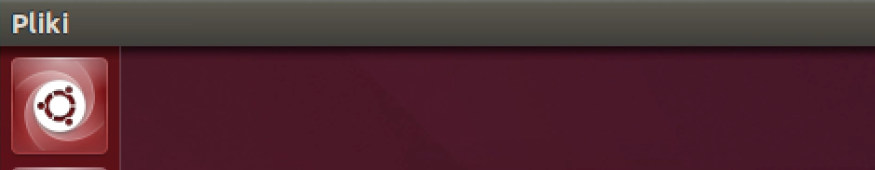
\includegraphics[width=\linewidth]{images/unity_menu_bar2.png}
\end{center}

Pasek menu jest wyświetlany, gdy kursor myszy znajdzie się nad panelem menu:

\begin{center}
	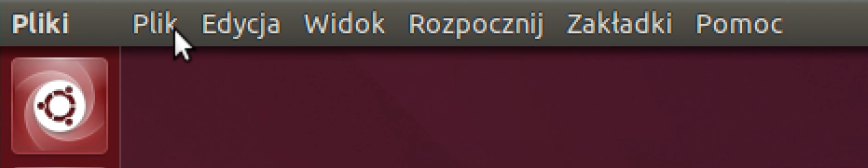
\includegraphics[width=\linewidth]{images/unity_menu_bar3.png}
\end{center}

Umieszczenie paska menu na panelu ma swoje plusy w przypadku urządzeń z ekranem ograniczonym niską rozdzielczością. Tak zwane \textcolor{ubuntu_orange}{Global Menu} pozwala lepiej wykorzystać miejsce dostępne w~pionie.
